\section{Edge Detection}
\begin{frame}{Edge Detection}
    \begin{figure}
        \centering
        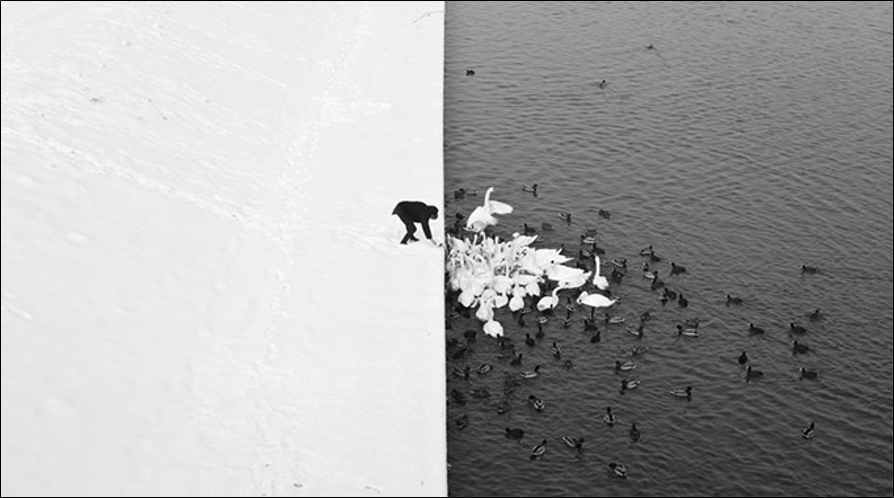
\includegraphics[width=0.8\textwidth]{imge0000.png}
        \caption{Winter in Krak{\'o}w photographed by Marcin Ryczek}\label{fi:ryczek}
    \end{figure}
\end{frame}


\begin{frame}{Edge detection}
    \begin{itemize}
    \item Goal:  Identify sudden changes (discontinuities) in an image
    \item Intuitively, edges carry most of the semantic and shape information from the image
    \end{itemize}
    {
        \centering
        \begin{tikzpicture}[scale=0.7]
\node[inner sep=0pt] (bottle) at (0,0)     {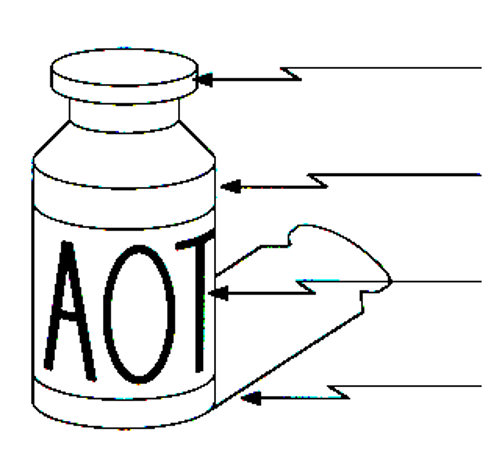
\includegraphics[scale=0.7]{edge_bottle.png}};
\draw (bottle.south east) ++ (0,1.4) node [anchor=west] {Illumination discontinuity};
\draw (bottle.south east) ++ (0,3.3) node [anchor=west] {Surface color discontinuity};
\draw (bottle.south east) ++ (0,5.1) node [anchor=west] {Depth discontinuity};
\draw (bottle.south east) ++ (0,6.9) node [anchor=west] {Surface normal discontinuity};
\end{tikzpicture} 
    }
    \credit{D. Lowe and S. Seitz}
\end{frame}


\begin{frame}{Edge detection}
    \begin{figure}[ht]
      \centering
      \begin{subfigure}[b]{0.3\textwidth}
        \centering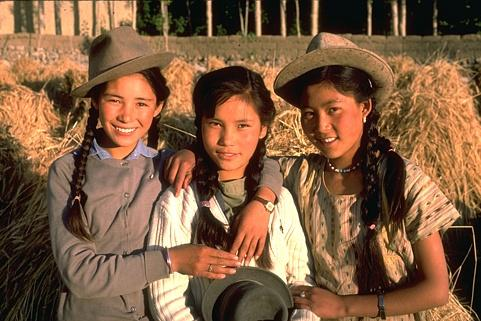
\includegraphics[width=\textwidth]{berkeley_376001_image.jpg}
        \caption{Image}\label{sf:galn}
      \end{subfigure}%   
      ~   
      \begin{subfigure}[b]{0.3\textwidth}
        \centering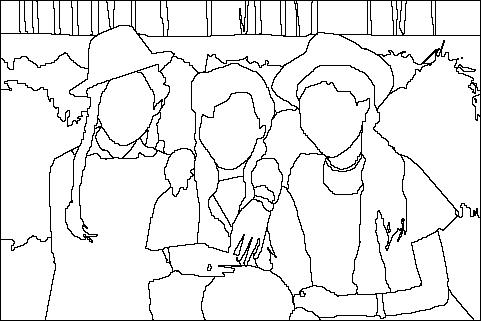
\includegraphics[width=\textwidth]{berkeley_376001_seg.jpg}
        \caption{A human's line drawing}\label{sf:galn}
      \end{subfigure}%
      ~
      \begin{subfigure}[b]{0.3\textwidth}
        \centering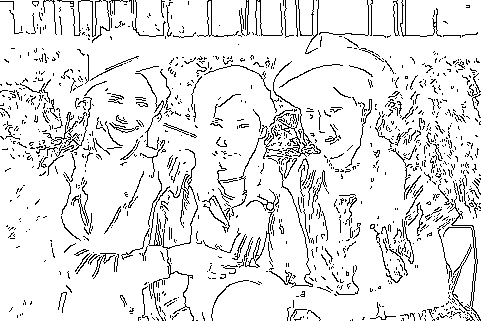
\includegraphics[width=\textwidth]{berkeley_376001_canny.jpg}
        \caption{Reality}\label{sf:galb}
      \end{subfigure}
      \caption{Edges: ideal vs. reality.}
    \end{figure}

\end{frame}



\begin{frame}
\frametitle{Edge detection}
\begin{itemize}
\item An edge is a place of rapid change in the image intensity function
\end{itemize}

\includegraphics{imge0003.png}
\begin{itemize}
\item image
\end{itemize}
%PartTitle:
%PartTitle:
%PartTitle:
%PartTitle: intensity function (along horizontal scanline)
%PartTitle:
%PartTitle:
%PartTitle:
%PartTitle: first derivative
%PartTitle:
%PartTitle:
%PartTitle: edges correspond to extrema of derivative

\end{frame}


\begin{frame}
\frametitle{Derivatives with convolution}
\begin{itemize}
\item For 2D function f(x,y), the partial derivative is:
\item
\item
\item
\item
\item For discrete data, we can approximate using finite differences:
\item
\item
\item
\item To implement the above as convolution, what would be  the associated filter?
\end{itemize}
\ includegraphics{imge0004.png}
\ includegraphics{imge0005.png}
\begin{itemize}
\item Source: K. Grauman
\end{itemize}

\end{frame}


\begin{frame}
\frametitle{Partial derivatives of an image}
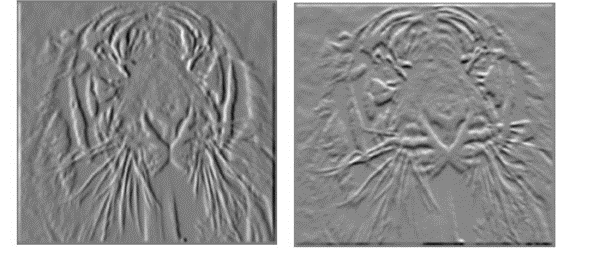
\includegraphics{imge0006.png}
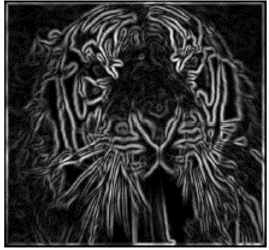
\includegraphics{imge0007.png}
\begin{itemize}
\item Which shows changes with respect to x?
\end{itemize}
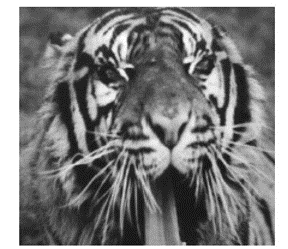
\includegraphics{imge0008.png}
%PartTitle: -1     1
%PartTitle: 1     -1
\begin{itemize}
\item or
\end{itemize}
%PartTitle: -1    1
\ includegraphics{imge0009.png}
\ includegraphics{imge0010.png}

\end{frame}


\begin{frame}
\frametitle{Finite difference filters}
\begin{itemize}
\item Other approximations of derivative filters exist:
\end{itemize}
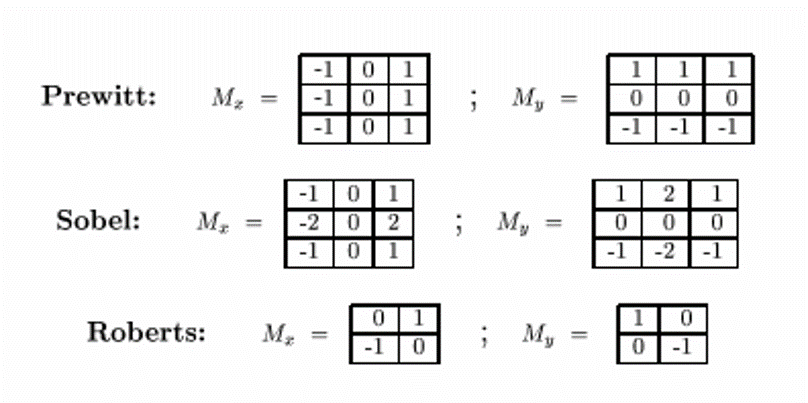
\includegraphics{imge0011.png}
\begin{itemize}
\item Source: K. Grauman
\end{itemize}

\end{frame}


\begin{frame}
\frametitle{Image gradient}
\begin{itemize}
\item The gradient points in the direction of most rapid increase in intensity
\end{itemize}
%PartTitle:
%PartTitle:
%PartTitle:
\begin{itemize}
\item The gradient of an image:
\item
\item
\item
\end{itemize}
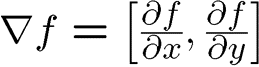
\includegraphics{imge0012.png}
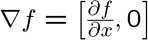
\includegraphics{imge0013.png}
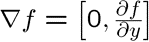
\includegraphics{imge0014.png}
%PartTitle:
%PartTitle:
%PartTitle:
\begin{itemize}
\item The gradient direction is given by
\end{itemize}
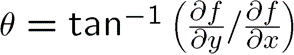
\includegraphics{imge0015.png}
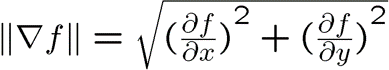
\includegraphics{imge0016.png}
\begin{itemize}
\item Source: Steve Seitz
\end{itemize}
\begin{itemize}
\item The edge strength is given by the gradient magnitude
\end{itemize}
\begin{itemize}
\item How does this direction relate to the direction of the edge?
\end{itemize}

\end{frame}


\begin{frame}
\frametitle{Application: Gradient-domain image editing}
\begin{itemize}
\item Goal: solve for pixel values in the target region to match gradients of the source region while keeping background pixels the same
\end{itemize}
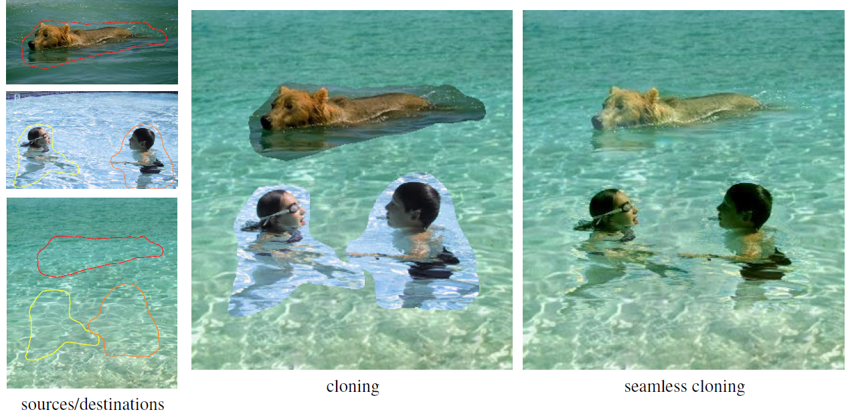
\includegraphics{imge0017.png}
\begin{itemize}
\item P. Perez, M. Gangnet, A. Blake, Poisson Image Editing, SIGGRAPH 2003
\end{itemize}

\end{frame}


\begin{frame}
\frametitle{Effects of noise}
\begin{itemize}
\item Consider a single row or column of the image
\end{itemize}
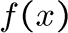
\includegraphics{imge0018.png}
%PartTitle: Where is the edge?
\begin{itemize}
\item Source: S. Seitz
\end{itemize}

\end{frame}


\begin{frame}
\frametitle{Solution: smooth first}
%PartTitle: To find edges, look for peaks in
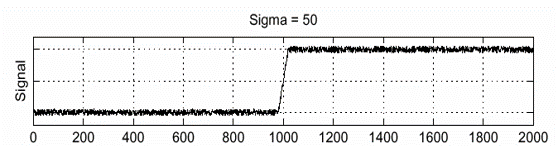
\includegraphics{imge0019.png}
\begin{itemize}
\item f
\end{itemize}
%PartTitle: g
%PartTitle: f * g
\begin{itemize}
\item Source: S. Seitz
\end{itemize}

\end{frame}


\begin{frame}
\frametitle{Derivative theorem of convolution}
\begin{itemize}
\item Differentiation is convolution, and convolution is associative:
\item This saves us one operation:
\end{itemize}
\ includegraphics{imge0020.png}
%PartTitle: f
\begin{itemize}
\item Source: S. Seitz
\end{itemize}

\end{frame}


\begin{frame}
\frametitle{Derivative of Gaussian filters}
\begin{itemize}
\item Which one finds horizontal/vertical edges?
\end{itemize}
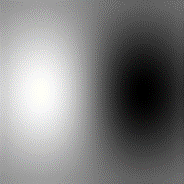
\includegraphics{imge0021.png}
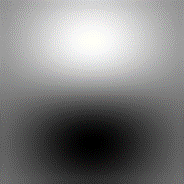
\includegraphics{imge0022.png}
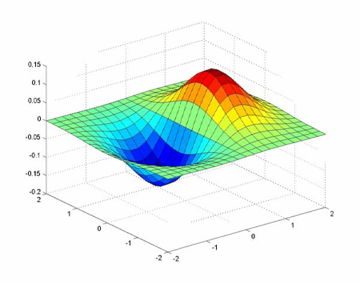
\includegraphics{imge0023.png}
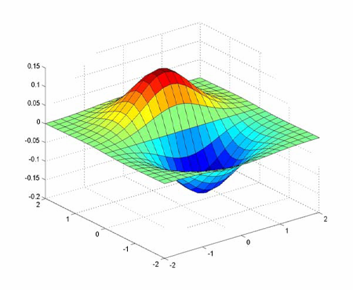
\includegraphics{imge0024.png}
\begin{itemize}
\item x-direction
\end{itemize}
\begin{itemize}
\item y-direction
\end{itemize}

\end{frame}


\begin{frame}
\frametitle{Derivative of Gaussian filters}
\begin{itemize}
\item Are these filters separable?
\end{itemize}
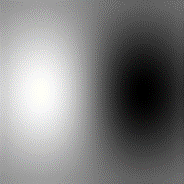
\includegraphics{imge0025.png}
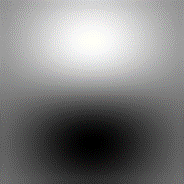
\includegraphics{imge0026.png}
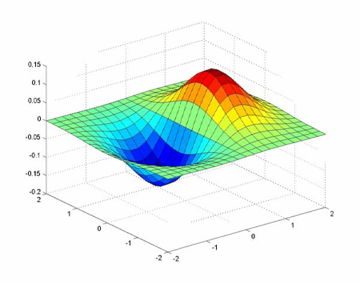
\includegraphics{imge0027.png}
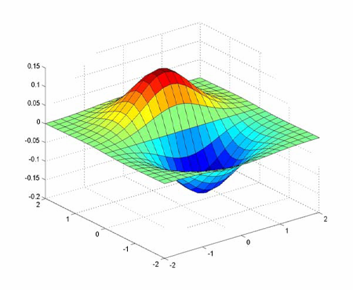
\includegraphics{imge0028.png}
\begin{itemize}
\item x-direction
\end{itemize}
\begin{itemize}
\item y-direction
\end{itemize}

\end{frame}


\begin{frame}
\frametitle{Recall: Separability of the Gaussian filter}
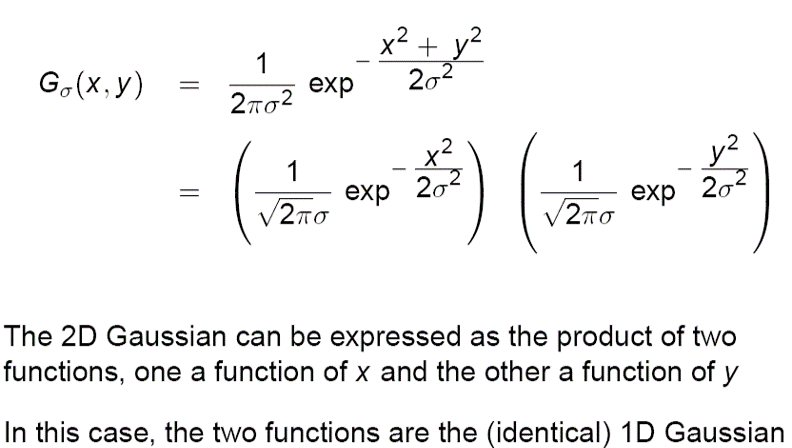
\includegraphics{imge0029.png}
\begin{itemize}
\item Source: D. Lowe
\end{itemize}

\end{frame}

